\chapter{Network Security: Crypto, TLS, and Firewalls}\label{ch:security}
\begin{quote}
\emph{``Security is not a feature you add; it is a property you prove.''} --- Every packet you send may cross a hostile network. This chapter builds defence from zero: what crypto guarantees, how TLS stitches those guarantees into HTTPS, and where firewalls and VPNs fit when crypto alone is not enough.
\end{quote}

\noindent\fbox{\parbox{\dimexpr\linewidth-2\fboxsep-2\fboxrule}{%
\textbf{From zero: we build here, no crypto background assumed.} We start with intuition---locked boxes and seal wax---then formalise: confidentiality, integrity, authentication. Each primitive is picture $\to$ words $\to$ definition, with Python you can run to see it fail when misused.}}%
\vspace{0.4em}

\section*{Learning Outcomes}
After this chapter you will be able to:
\begin{enumerate}[label=(L\arabic*)]
    \item distinguish confidentiality, integrity, authentication and non-repudiation;
    \item compare symmetric vs.\ public-key crypto and explain key distribution;
    \item use hashes, MACs and digital signatures to detect tampering;
    \item walk through a TLS 1.2/1.3 handshake and explain certificates;
    \item place firewalls, IDS and VPNs in a layered defence and name their limits.
\end{enumerate}

% ============================================================
\section{What Security Means: CIA and Threat Model}\label{sec:cia}
Picture sending a letter: you want no one but the recipient to read it (confidentiality), no one to alter it in transit (integrity), the recipient to be sure it came from you (authentication), and to be unable to deny it later (non-repudiation). Networks add an attacker who can \emph{eavesdrop}, \emph{modify}, \emph{inject}, and \emph{replay} packets anywhere on the path.

We formalise with a threat model: Dolev-Yao attacker controls the network (reads, drops, reorders every packet) but cannot break crypto without the key. Goals are CIA plus availability. Attacks: sniffing (passive read), spoofing/IP spoofing, man-in-the-middle (MITM), replay, denial-of-service. Defence is layered: crypto at the ends, firewalls at the borders, monitoring everywhere.

\begin{figure}[h]
\centering
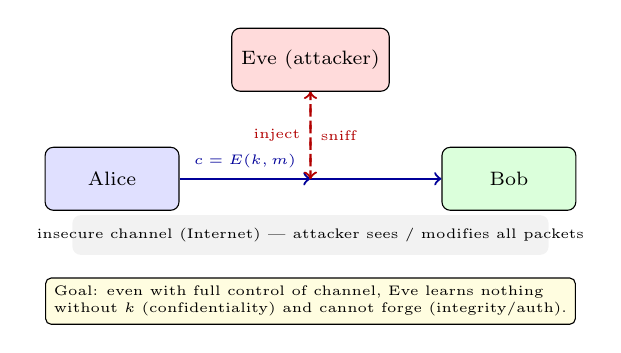
\begin{tikzpicture}[scale=0.84,every node/.style={font=\scriptsize}]
% Alice, Bob, Eve
\node[draw,fill=blue!12,rounded corners=3pt,minimum width=1.7cm,minimum height=0.8cm] (alice) at (0,0) {Alice};
\node[draw,fill=green!14,rounded corners=3pt,minimum width=1.7cm,minimum height=0.8cm] (bob) at (6,0) {Bob};
\node[draw,fill=red!14,rounded corners=3pt,minimum width=2.0cm,minimum height=0.8cm] (eve) at (3,1.8) {Eve (attacker)};
% Channel
\fill[gray!10,rounded corners=3pt] (-0.6,-0.55) rectangle (6.6,-1.15);
\node[font=\tiny] at (3,-0.85) {insecure channel (Internet) --- attacker sees / modifies all packets};
\draw[->,thick,blue!60!black] (alice.east) -- (3,0) node[midway,above,font=\tiny] {$c=E(k,m)$};
\draw[->,thick,blue!60!black] (3,0) -- (bob.west);
% Eve taps
\draw[->,thick,red!70!black,dashed] (3,0) -- (eve.south) node[midway,right,font=\tiny] {sniff};
\draw[->,thick,red!70!black,dashed] (eve.south) -- (3,0) node[midway,left,font=\tiny] {inject};
% Goals
\node[font=\tiny,fill=yellow!12,draw,rounded corners=2pt,inner sep=3pt,align=left] at (3,-1.85) {Goal: even with full control of channel, Eve learns nothing\\without $k$ (confidentiality) and cannot forge (integrity/auth).};
\end{tikzpicture}
\caption{Threat model: Eve controls the channel between Alice and Bob. Crypto must protect $m$ even though $c$ is fully exposed.}
\label{fig:threat-model}
\end{figure}

\section{Symmetric Cryptography}\label{sec:symmetric}
One key $k$ locks and unlocks. Intuition: a single padlocked box where both sides share the key.

Formally, encryption $c=E(k,m)$, decryption $m=D(k,c)$ with $D(k,E(k,m))=m$. Security means without $k$, $c$ reveals nothing about $m$ (indistinguishability). Two families:

\textbf{Stream ciphers} XOR a keystream $S(k,\text{nonce})$ with plaintext: $c=m\oplus S$. If nonce repeats, $c_1\oplus c_2=m_1\oplus m_2$ leaks. \textbf{Block ciphers} (AES-128/256) encrypt fixed 128-bit blocks; longer messages need a mode: CBC, CTR, or GCM (which adds integrity). Never use ECB (identical plaintext blocks $\to$ identical ciphertext blocks).

Key size matters: AES-128 has $2^{128}$ keys; brute force is infeasible, but a 40-bit key falls in hours. Key distribution is the pain: how do Alice and Bob share $k$ without Eve reading it? That needs public-key crypto.

\begin{lstlisting}[language=Python]
# Toy demo: AES-like usage via Python's toy XOR (do NOT use raw XOR in production!)
import os, hashlib
def xor_stream(key: bytes, nonce: bytes, msg: bytes) -> bytes:
    # keystream = SHA256(key||nonce||counter) repeated
    ks = b""
    for ctr in range((len(msg)+31)//32):
        ks += hashlib.sha256(key + nonce + ctr.to_bytes(4,'big')).digest()
    return bytes(a^b for a,b in zip(msg, ks[:len(msg)]))

key = os.urandom(16); nonce = os.urandom(8)
msg = b"Transfer $100 to Bob"
ct = xor_stream(key, nonce, msg)
pt = xor_stream(key, nonce, ct)  # decrypt = same XOR
assert pt == msg
# Reusing nonce leaks: ct1 ^ ct2 == msg1 ^ msg2
ct2 = xor_stream(key, nonce, b"Transfer $900 to Eve")
leak = bytes(a^b for a,b in zip(ct, ct2))  # == msg ^ msg2
\end{lstlisting}

Hashes and MACs are next; they do not encrypt but ensure nothing changed.

\section{Hashes, MACs, and Signatures}\label{sec:hash-mac}
A \emph{cryptographic hash} $H(m)$ is a fixed-size fingerprint (e.g., SHA-256 $\to$ 256 bits) that is preimage-resistant (given $h$, cannot find $m$), second-preimage resistant, and collision-resistant. Even one-bit change flips $\approx$ half the output bits.

A \emph{MAC} (message authentication code) adds a key: $\text{MAC}=H(k\parallel m)$ in toy form, real HMAC is $H((k\oplus\text{opad})\parallel H((k\oplus\text{ipad})\parallel m))$. Receiver recomputes and compares; mismatch means tampering or wrong key. Hash alone does not authenticate: Eve can replace $(m, H(m))$ with $(m', H(m'))$.

\emph{Digital signatures} give public verifiability and non-repudiation via public-key crypto: Alice signs with private key, anyone verifies with public key, but only Alice could have signed.

\begin{figure}[h]
\centering
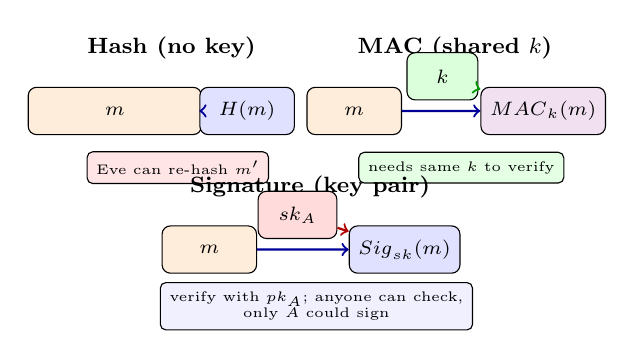
\begin{tikzpicture}[scale=0.80,every node/.style={font=\scriptsize}]
% Hash vs MAC vs Signature
\begin{scope}
\node[font=\footnotesize\bfseries] at (1.6,2.0) {Hash (no key)};
\node[draw,fill=orange!14,rounded corners=3pt,minimum width=2.2cm,minimum height=0.6cm] (m1) at (0.7,1.0) {$m$};
\node[draw,fill=blue!12,rounded corners=3pt,minimum width=1.2cm,minimum height=0.6cm] (h1) at (2.8,1.0) {$H(m)$};
\draw[->,thick,blue!60!black] (m1) -- (h1);
\node[font=\tiny,fill=red!10,draw,rounded corners=2pt] at (1.7,0.1) {Eve can re-hash $m'$};
\end{scope}
\begin{scope}[xshift=4.5cm]
\node[font=\footnotesize\bfseries] at (1.6,2.0) {MAC (shared $k$)};
\node[draw,fill=orange!14,rounded corners=3pt,minimum width=1.2cm,minimum height=0.6cm] (m2) at (0,1.0) {$m$};
\node[draw,fill=green!14,rounded corners=3pt,minimum width=0.9cm,minimum height=0.6cm] (k2) at (1.4,1.55) {$k$};
\node[draw,fill=violet!12,rounded corners=3pt,minimum width=1.2cm,minimum height=0.6cm] (t2) at (3.0,1.0) {$\text{MAC}_k(m)$};
\draw[->,thick,blue!60!black] (m2) -- (t2);
\draw[->,thick,green!60!black] (k2) -- (t2);
\node[font=\tiny,fill=green!10,draw,rounded corners=2pt] at (1.7,0.1) {needs same $k$ to verify};
\end{scope}
\begin{scope}[yshift=-2.2cm,xshift=2.2cm]
\node[font=\footnotesize\bfseries] at (1.6,2.0) {Signature (key pair)};
\node[draw,fill=orange!14,rounded corners=3pt,minimum width=1.2cm,minimum height=0.6cm] (m3) at (0,1.0) {$m$};
\node[draw,fill=red!14,rounded corners=3pt,minimum width=1.0cm,minimum height=0.6cm] (sk) at (1.4,1.55) {$sk_A$};
\node[draw,fill=blue!12,rounded corners=3pt,minimum width=1.3cm,minimum height=0.6cm] (sig) at (3.1,1.0) {$\text{Sig}_{sk}(m)$};
\draw[->,thick,blue!60!black] (m3) -- (sig);
\draw[->,thick,red!70!black] (sk) -- (sig);
\node[font=\tiny,align=center,fill=blue!6,draw,rounded corners=2pt] at (1.7,0.1) {verify with $pk_A$; anyone can check,\\only $A$ could sign};
\end{scope}
\end{tikzpicture}
\caption{Hash detects accidental change; MAC detects tampering with a shared key; signature does it with a key pair and adds non-repudiation.}
\label{fig:hash-mac-sig}
\end{figure}

\section{Public-Key Crypto and Key Exchange}\label{sec:pubkey}
Two keys: public $pk$ (share widely) and private $sk$ (never share). $c=E(pk,m)$, $m=D(sk,c)$. Analogy: an open padlock (pk) anyone can snap shut, but only you have the key (sk) to open.

\textbf{RSA} (Rivest-Shamir-Adleman): pick large primes $p,q$, $n=pq$, choose $e$ coprime to $\phi(n)=(p-1)(q-1)$, compute $d=e^{-1}\bmod\phi(n)$. Then $pk=(e,n)$, $sk=(d,n)$, $E(m)=m^e\bmod n$, $D(c)=c^d\bmod n$. Security relies on factoring $n$ being hard.

\textbf{Diffie-Hellman} lets Alice and Bob agree on a shared secret over a public channel: agree on prime $p$ and generator $g$; Alice picks $a$, sends $A=g^a\bmod p$; Bob picks $b$, sends $B=g^b\bmod p$; both compute $s=B^a=A^b=g^{ab}\bmod p$. Eve sees $A,B,g,p$ but not $a,b$, and computing $g^{ab}$ is believed hard (discrete log).

\begin{lstlisting}[language=Python]
# Tiny RSA demo (toy primes -- real RSA uses 2048-bit primes!)
import math
p, q = 61, 53
n = p*q; phi = (p-1)*(q-1)
e = 17  # coprime to phi
d = pow(e, -1, phi)  # modular inverse (Python 3.8+)
print(f"pk=({e},{n}) sk=({d},{n})")
def rsa_encrypt(m, e, n): return pow(m, e, n)
def rsa_decrypt(c, d, n): return pow(c, d, n)
msg = 42
ct = rsa_encrypt(msg, e, n); pt = rsa_decrypt(ct, d, n)
assert pt == msg, "RSA round-trip failed"
print(f"msg {msg} -> ct {ct} -> pt {pt}")

# Diffie-Hellman (tiny p for demo)
p_dh, g = 23, 5
a, b = 6, 15
A = pow(g, a, p_dh); B = pow(g, b, p_dh)
s_alice = pow(B, a, p_dh); s_bob = pow(A, b, p_dh)
assert s_alice == s_bob
print(f"DH shared secret: {s_alice}")
\end{lstlisting}

RSA is slow ($\approx 1000\times$ slower than AES) so we use hybrid: RSA or DH to exchange a short AES key, then AES for bulk data. The signature direction is reversed: sign with $sk$, verify with $pk$.

\section{TLS: How HTTPS Works}\label{sec:tls}
TLS stitches everything: authentication via certificates, key exchange via (EC)DHE or RSA, bulk encryption via AES/ChaCha, integrity via MAC/GCM. TLS 1.3 removed RSA key transport and static DH to enforce forward secrecy.

Simplified handshake (TLS 1.2/1.3 core):

\begin{enumerate}[itemsep=0.3em]
    \item ClientHello: client nonce $r_C$, offered ciphers, key share.
    \item ServerHello: server nonce $r_S$, chosen cipher, key share, Certificate (chain to trusted CA), ServerKeyExchange if needed.
    \item Client verifies certificate (CA signature, hostname, expiry, revocation), computes premaster, derives session keys via PRF/hash.
    \item Both send Finished (MAC over transcript) to confirm no tampering or downgrade.
\end{enumerate}

\begin{figure}[h]
\centering
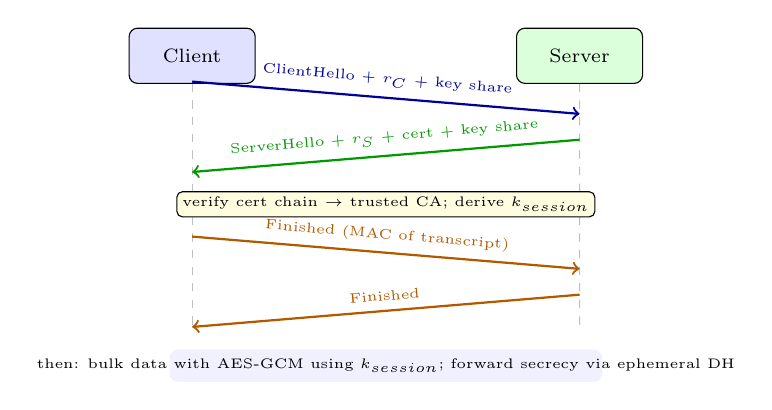
\begin{tikzpicture}[scale=0.82,every node/.style={font=\scriptsize}]
\node[draw,fill=blue!12,rounded corners=3pt,minimum width=1.6cm,minimum height=0.7cm] (cli) at (0,4.2) {Client};
\node[draw,fill=green!14,rounded corners=3pt,minimum width=1.6cm,minimum height=0.7cm] (srv) at (6,4.2) {Server};
\draw[dashed,gray!50] (cli.south) -- (0,0);
\draw[dashed,gray!50] (srv.south) -- (6,0);
% Messages
\draw[->,thick,blue!60!black] (0,3.8) -- (6,3.3) node[midway,above,sloped,font=\tiny] {ClientHello + $r_C$ + key share};
\draw[->,thick,green!60!black] (6,2.9) -- (0,2.4) node[midway,above,sloped,font=\tiny] {ServerHello + $r_S$ + cert + key share};
\node[font=\tiny,fill=yellow!12,draw,rounded corners=2pt,inner sep=2pt] at (3,1.9) {verify cert chain $\to$ trusted CA; derive $k_{\text{session}}$};
\draw[->,thick,orange!70!black] (0,1.4) -- (6,0.9) node[midway,above,sloped,font=\tiny] {Finished (MAC of transcript)};
\draw[->,thick,orange!70!black] (6,0.5) -- (0,0.0) node[midway,above,sloped,font=\tiny] {Finished};
% Data
\fill[blue!6,rounded corners=3pt] (-0.35,-0.85) rectangle (6.35,-0.35);
\node[font=\tiny] at (3,-0.60) {then: bulk data with AES-GCM using $k_{\text{session}}$; forward secrecy via ephemeral DH};
\end{tikzpicture}
\caption{TLS handshake (simplified): nonces + key shares $\to$ session key, certificate authenticates server, Finished confirms integrity.}
\label{fig:tls-handshake}
\end{figure}

Now application data flows encrypted and integrity-protected. Certificates bind $pk$ to a domain; a CA signs the binding. Browser ships $\approx 100$ trusted CA roots; compromise of any CA breaks trust, hence Certificate Transparency logs.

\section{Firewalls, IDS, and VPNs}\label{sec:firewalls}
Crypto protects data in transit; firewalls control \emph{who} can connect at network borders.

\textbf{Packet filter} (stateless): rules on 5-tuple (src IP, dst IP, src port, dst port, protocol). Example: block inbound TCP SYN to port 22 except from 137.132.0.0/16. Cheap but cannot track connections.

\textbf{Stateful filter}: tracks TCP state (SYN, ESTABLISHED); allows inbound only if matching outbound established. Handles FTP active mode and tolerates ephemeral ports.

\textbf{Application gateway / proxy}: terminates connection, inspects application payload (e.g., HTTP filtering). Stronger but slower.

Placement: a \emph{DMZ} between outer and inner firewalls hosts public servers (web, mail); inner firewall protects the private LAN. \emph{IDS} (intrusion detection) sniffs and alerts on signatures or anomalies; \emph{IPS} blocks inline. They do not replace crypto: a firewall cannot stop a phished password or a malicious insider; it just shrinks the reachable attack surface.

\textbf{VPN} (virtual private network) tunnels private traffic over the public Internet: IPSec at IP layer (tunnel vs.\ transport mode) or TLS-VPN at application layer. Site-to-site IPSec uses ESP (encrypted payload + integrity); remote-access VPN authenticates the user then assigns a virtual IP.

\section{Putting It Together: Why TLS Alone Is Not Enough}\label{sec:together}
TLS gives confidentiality and server authentication on one connection, but says nothing about what the server does with $m$ afterwards (database breach, XSS, insider). Firewalls limit who reaches the TLS terminator, IDS spots brute-force and scans, and key management (rotation, HSM, least privilege) limits blast radius when a key leaks. Security is a chain: weakest link---often human (phishing, reuse of passwords, misconfigured S3 bucket)---breaks it regardless of cipher strength. Hence defence in depth: harden each layer and assume breach.

\section{Chapter Notes}
Schneier, Katz \& Lindell, and Kurose \& Ross Ch.~8 cover this material. For hands-on, try Wireshark to inspect a real TLS handshake and \texttt{iptables} / \texttt{nft} to write a stateful rule set; the gap between textbook and real config is where exams and interviews probe.

\section{Exercises}\label{sec:ch08-exercises}
\begin{enumerate}[label=E8.\arabic*, leftmargin=*, itemsep=0.8em]
    \item \textbf{CIA mapping.} For each scenario---(a) sniffing unencrypted HTTP, (b) altering DNS reply, (c) forging a grade-submission email---state which of confidentiality, integrity, authentication or non-repudiation fails and which crypto primitive (encryption, MAC, signature, cert) fixes it.
    \item \textbf{RSA by hand.} With $p=5,q=11,e=3$ compute $n,\phi(n),d$ and encrypt $m=6$ then decrypt. Show what goes wrong if you reuse $k$ or use ECB mode for AES on an image (describe the visible artefact).
    \item \textbf{Hash vs.\ MAC vs.\ signature.} Alice sends $(m,H(m))$ without a key. Show Eve's exact forging steps. Then show why HMAC-SHA256 with a shared key stops forging but still allows Alice to deny sending $m$; explain how signing with $sk_A$ fixes non-repudiation.
    \item \textbf{TLS trace.} List every TLS 1.2 message from ClientHello to Finished for a fresh connection to \texttt{example.com}. Mark which are encrypted, which prove possession of the server private key, and which provide forward secrecy when (EC)DHE is used vs.\ RSA key transport.
    \item \textbf{Firewall rules.} Write a stateful rule set: allow outbound HTTP/HTTPS/DNS, allow inbound only for established connections, block inbound SSH except from campus 137.132.0.0/16, and place a web server in a DMZ. Explain each rule and give a packet that is blocked and one that passes, plus what IDS would catch that the firewall misses.
\end{enumerate}
% End of Chapter 8
